\documentclass[fontset=windows,pass]{article}
\usepackage[margin=1in]{geometry}%设置边距,符合Word设定
\usepackage{ctex}
\usepackage{setspace}
\usepackage{lipsum}
\usepackage{graphicx}%插入图片
\usepackage{amsmath}
\usepackage{amssymb}
\usepackage{mathrsfs}
\numberwithin{equation}{subsection} % 使公式编号依赖于章节
\graphicspath{{Figures/}}%文章所用图片在当前目录下的 Figures目录

\renewcommand{\contentsname}{\centerline{Contents}} %经过设置word格式后,将目录标题居中


\title{\heiti\zihao{2} Machine Learning}
\author{\songti Bruce Zhang}
\date{2024.12.3}


\begin{document}
	\maketitle
	\thispagestyle{empty}

\tableofcontents

\newpage
\section{What is Machine Learning?}
Typically, Machine Learning is divided into two kinds of parts, Supervised learning and
Unsupervised learning.

\textbf{Supervised learning: Learns from being given "right answers".}
\[
\text{Supervised learning} =
\begin{cases}
\text{Regression(回归): Predict a number, infinitely many possible outputs.}\\
\text{Classification(分类): Predict categories, small number of possible outputs.}
\end{cases}
\]

\textbf{Unsupervised learning: Data only comes with inputs x, but not outputs labels y. Algorithm
has to find structure in the data.}
\[
\text{Unsupervised learning} = 
\begin{cases}
	\text{Clustering(聚类): Group similar data points together.}\\
	\text{Dimensionality reduction(降维): Compress data using fewer number.}\\
	\text{Anomaly detection(异常检测): Find unusual data points.}
\end{cases}
\]

\section{Supervised Learning}
The main \textbf{notation} we will use are as follows
\begin{align*}
	x & = \text{"input" variable or "input" feature} \\
	y & = \text{"target" variable or "output" variable} \\
	m & = \text{number of training examples} \\
	(x^{(i)}, y^{(i)}) & = \text{$i^{\text{th}}$ training examples}
\end{align*}

Seen pictorially, the process is therefore like this:

\begin{center}
	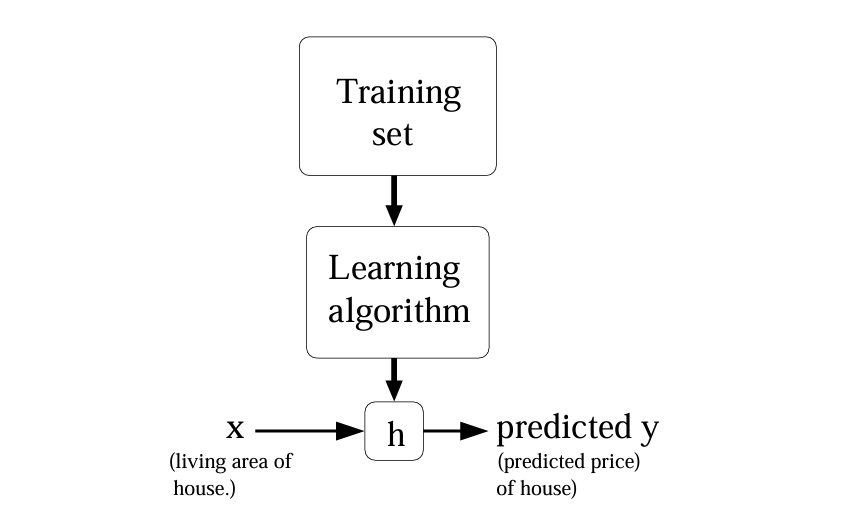
\includegraphics[width = 0.8\textwidth]{Figures/Supervised_Method.png}
\end{center}

When the target variable that we're trying to predict is continuous, such as in our housing example, 
we call the learning problem a \textbf{regression} problem. When y can take on only a small number of discrete values 
(such as if, given the living area, we wanted to predict if a dwelling is a house or an
 apartment, say), we call it a \textbf{classification} problem.

\subsection{Linear Regression}

\[
\begin{array}{c|c|c}
\textbf{Living area (feet$^2$)} & \textbf{\#bedrooms} & \textbf{Price (1000\$s)} \\
\hline
2104 & 3 & 400 \\
1600 & 3 & 330 \\
2400 & 3 & 369 \\
1416 & 2 & 232 \\
3000 & 4 & 540 \\
\vdots & \vdots & \vdots \\
\end{array}
\]

Given this training set, obvisouly, the input feature, namely the $\boldsymbol{x}$ is two-dimensional vector
in $\mathbb{R}^2$. Recalling the previous picture, what we need to do is representing a function
h, which predicts the output $\hat{y}$. Let's say we decide to approximate $y$ as a linear function of $x$:

\begin{equation}
	h_\theta(x) = \theta_0 + \theta_1 x_1 + \theta_2 x_2
\end{equation}

The $\theta_i$'s are the parameters (also called \textbf{weight}) parameterizing the space of linear functions.
To simplify our notation, we introduce the convention of letting $x_0 = 1$ (\textbf{intercept term}).

\[
	h(\boldsymbol{x}) = \sum_{i=0}^{n} \theta_i x_i = \boldsymbol{\theta}^T \boldsymbol{x}
\]

A problem is that how can we identify the parameters so that the output of $h(x)$, $\hat{y}$ close to $y$.
\textbf{So we actually need another function that can help us to evaluate how good a $\boldsymbol{\theta}$ parameter-based function is}.
We define the \textbf{cost function}:

\begin{equation}
	J(\boldsymbol{\theta}) = \frac{1}{2m} \sum_{i=1}^{m} \left(h(x^{(i)})-y^{(i)}\right)^2
\end{equation}

\subsubsection{Gradient Descent Algorithm}

Just like the name of "cost function", we hope to choose $\boldsymbol{\theta}$ so as to 
minimize $J(\boldsymbol{\theta})$. What we really want is an efficient algorithm that we can write
in code for automatically finding the values of parameters $\boldsymbol{\theta}$, they give us the
best fit line, that minimizes the cost function $J$.

Let's consider the \textbf{gradient descent algorithm}, which start with some initial $\boldsymbol{\theta}$, and 
repeatedly performs the update:

\begin{equation}
	\boldsymbol{\theta}_j = \boldsymbol{\theta}_j-\alpha \frac{\partial}{\partial \boldsymbol{\theta}_j} J(\boldsymbol{\theta}) 
\end{equation}

$\alpha$ is called the \textbf{learning rate}.

(Note: This update is simultaneously performed for all values of $j = 0, \dots, n$.)


\begin{align*}
	\frac{\partial}{\partial \boldsymbol{\theta}_j} J(\boldsymbol{\theta}) & = \frac{1}{2m} \frac{\partial}{\partial \boldsymbol{\theta}_j}\
				\left[\sum_{i=1}^{m} \left(h(x^{(i)})-y^{(i)}\right)^2\right]\\
	& = \frac{1}{2m} \sum_{i=1}^{m}  \frac{\partial}{\partial \boldsymbol{\theta}_j} \left(h(x^{(i)})-y^{(i)}\right)^2\\
	& = \frac{1}{m} \sum_{i=1}^{m} \left(h(x^{(i)})-y^{(i)}\right) x^{(i)}_{j}
\end{align*}

In conclusion, this gives the update rule:

\begin{equation}
	\boldsymbol{\theta}_j = \boldsymbol{\theta}_j + \alpha \frac{1}{m} \sum_{i=1}^{m} \left[\left(y^{(i)} - h(x^{(i)})\right) x^{(i)}_{j}\right]
\end{equation}

The rule is called the \textbf{LMS} update rule (LMS stands for “least mean squares”),
and is also known as the \textbf{Widrow-Hoff} learning rule.

When I was reading the explanation of the equation above from the note of CS-229, I prefer Andrew Ng's
explanation in the video of Coursera.

In a moment, if the partial of $J$ is a positive number in a place, obvisouly with the increase of the parameter
$\theta_j$, the value of $J$ will alse increase, thus we minus this positive number so that the value of $J$ will decrease.
Accordingly, if the partial of $J$ is a negative number in a place, with the increase of the parameter
$\theta_j$, the value of $J$ will decrease, thus we minus this negative number so that the value of $J$ will decrease.

\begin{center}
	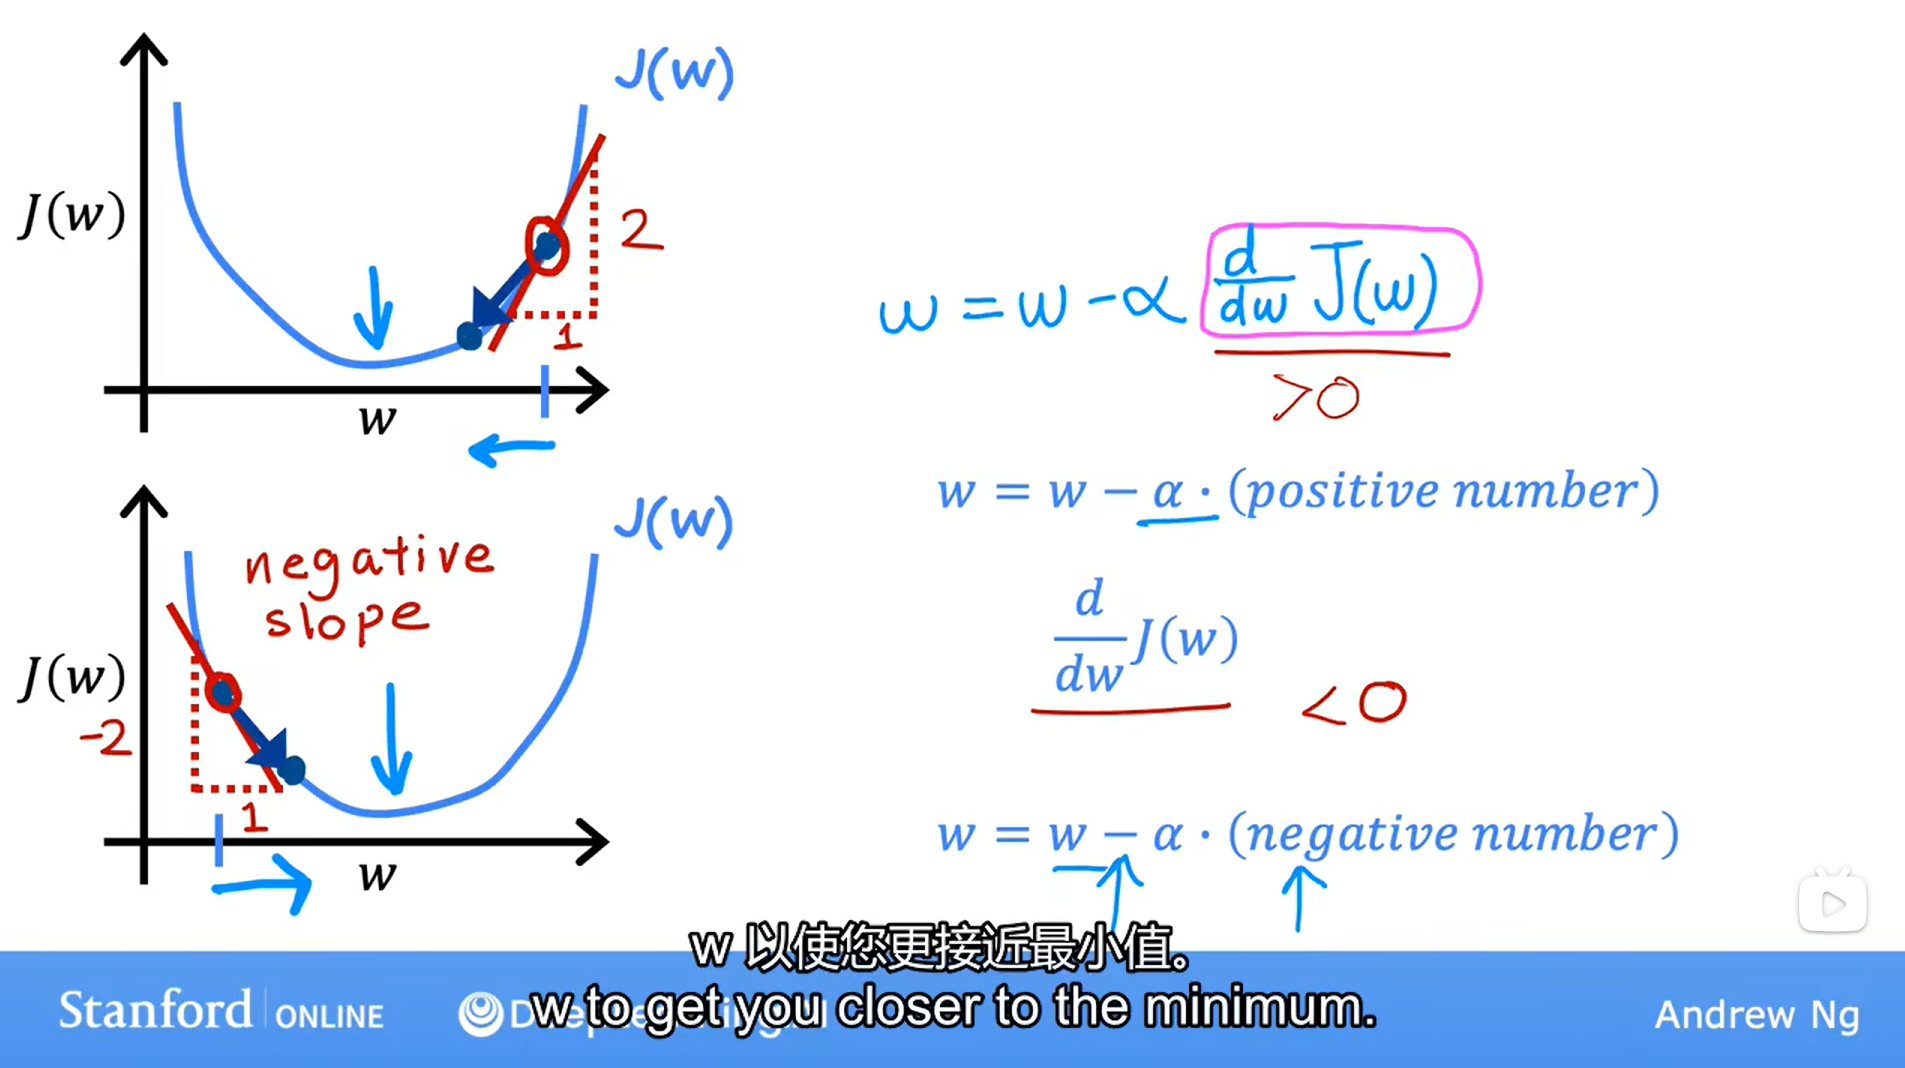
\includegraphics[width = 0.8\textwidth]{Figures/Gradient_Explanation.png}
\end{center}

This method looks at every example in the entire training set on every step, and is called \textbf{batch gradient descent}.
In fact, no mater where the initial value is chosen,  the optimization problem we have posed here
for linear regression has only one global, and no other local, optima, thus gradient descent always converges
because $J$ \textbf{is a convex quadratic function}.

There is an alternative to batch gradient descent that also works very well. Consider the following algorithm:

\[
\begin{aligned}
&\text{Loop } \{ \\
&\quad \text{for } i = 1 \text{ to } m, \{ \\
&\quad \quad \theta_j = \theta_j + \alpha \big(y^{(i)} - h_\theta(x^{(i)})\big) x_j^{(i)} \quad \text{(for every \( j \))}. \\
&\quad \} \\
&\}
\end{aligned}
\]

In this algorithm, we repeatedly run through the training set, and each time we encounter a training example, 
we update the parameters according to the gradient of the error with respect to that single training example only.
This algorithm is called \textbf{stochastic gradient descent} (also incremental gradient descent).
Whereas batch gradient descent has to scan through the entire training set before taking a single step—a costly operation 
if m is large—stochastic gradient descent can start making progress right away, and continues to make progress with each example it looks at. 
Often, stochastic gradient descent gets $\theta$ “close” to the minimum much faster than batch gradient descent.

\subsubsection{The Normal Equation}

Gradient descent gives one way of minimizing $J$. And it is time to perform the minimization explicitly and
without resorting to an iterative algorithm by explicitly taking $J$'s derivatives with respect to the $\theta_j$'s, and setting them to
zero.However, we need to introduce some notation before showing.

\begin{flushleft}
	{\Large \textbf{Matrix derivatives}}
\end{flushleft}

For a function $f$: $\mathbb{R}^{m \times n} \to \mathbb{R}$ mapping from $m$-by-$n$ matrices to the real numbers,
we define the derivative of $f$ with respect to $A$ to be:

\begin{equation}
	\nabla_A f(A) = 
	\begin{bmatrix}
	\frac{\partial f}{\partial A_{11}} & \cdots & \frac{\partial f}{\partial A_{1n}} \\
	\vdots & \ddots & \vdots \\
	\frac{\partial f}{\partial A_{m1}} & \cdots & \frac{\partial f}{\partial A_{mn}}
	\end{bmatrix}
\end{equation}

We also introduce the \textbf{trace} operator. For an square matrix $A$, the trace of $A$ is defined
to be the sum of its diagonal entries:

\[
	tr A = \sum_{i=1}^{n}A_{ii}
\]

There are lots of properties of the trace operator.
\begin{align*}
	tr AB & = tr BA\\
	tr A & = tr A^T\\
	tr (A+B) & = tr A + tr B\\
	tr aA & = atr A\\
	\nabla_A tr AB & = B^T\\
	\nabla_{A^T} f(A) & = \left(\nabla_A f(A)\right)^T\\
	\nabla_A tr AB{A^T}C & = CAB + C^TA{B^T}\\
	\nabla_A \left|A\right| & = \left|A\right| \left(A^{-1}\right)^T
\end{align*}

\begin{flushleft}
	{\Large \textbf{Least squares revisited}}
\end{flushleft}

Given a training set, define the design matrix X to be the m-by-n matrix that contains the training examples'
input values in its rows:

\[
	X = \begin{bmatrix}
		-\left(x^{(1)}\right)^T-\\
		-\left(x^{(2)}\right)^T-\\
		\vdots\\
		-\left(x^{(m)}\right)^T-\\
	\end{bmatrix}
\]

$\boldsymbol{y}$ is the m-dimensional vector containing all the target values from the training set:

\[
	\boldsymbol{y} = \begin{bmatrix}
		y^{(1)}\\
		y^{(2)}\\
		\vdots\\
		y^{(m)}\\
	\end{bmatrix}
\]

Notice that $h(x^{(i)}) = \left(x^{(i)}\right)^T \theta$:

\begin{align*}
	X \theta - \boldsymbol{y} & = \begin{bmatrix}
		\left(x^{(1)}\right)^T \theta\\
		\vdots\\
		\left(x^{(m)}\right)^T \theta
	\end{bmatrix} 
	- \begin{bmatrix}
		y^{(1)}\\
		\vdots\\
		y^{(m)}
	\end{bmatrix} = \begin{bmatrix}
		h(x^{(1)}) - y^{(1)}\\
		\vdots\\
		h(x^{(m)}) - y^{(m)}
	\end{bmatrix}
\end{align*}

using the fact that for a vector $z$, we have that $z^T z = \sum_{i}^{} z_i^2$:

\begin{align*}
	\frac{1}{2m} \left(X \theta - \boldsymbol{y}\right)^T \left(X \theta - \boldsymbol{y}\right) & = 
	\frac{1}{2m} \sum_{i=1}^{m} \left(h(x^{(i)}) - y^{(i)}\right)^2 \\
	& = J(\theta)
\end{align*}

Finally, to minimize J, let's find its derivatives with respect to $\theta$. Combining some of the previous function,
we find that

\begin{equation}
	\nabla_{A^T} tr ABA^{T}C = B^{T}A^{T}C^{T} + BA^{T}C
\end{equation}

Hence,

\begin{align*}
		\nabla_{\theta} J(\theta) & = \nabla_{\theta} \frac{1}{2m}(X \theta-\vec{y})^{T}(X \theta-\vec{y}) \\
		                          & = \frac{1}{2m} \nabla_{\theta}\left(\theta^{T} X^{T} X \theta-\theta^{T} X^{T} \vec{y}-\vec{y}^{T} X \theta+\vec{y}^{T} \vec{y}\right) \\
		                          & = \frac{1}{2m} \nabla_{\theta} \operatorname{tr}\left(\theta^{T} X^{T} X \theta-\theta^{T} X^{T} \vec{y}-\vec{y}^{T} X \theta+\vec{y}^{T} \vec{y}\right) \\
		                          & = \frac{1}{2m} \nabla_{\theta}\left(\operatorname{tr} \theta^{T} X^{T} X \theta-2 \operatorname{tr} \vec{y}^{T} X \theta\right) \\
		                          & = \frac{1}{2m}\left(X^{T} X \theta+X^{T} X \theta-2 X^{T} \vec{y}\right) \\
		                          & = X^{T} X \theta-X^{T} \vec{y}
\end{align*}

(IN FACT, I don't want to explain the details of the deduce, refering to CS229-note1)

To minimize J, we set its derivatives to zero, and obtain the \textbf{normal equation}:

\begin{equation}
	X^{T}X\theta = X^{T}\vec{y}
\end{equation}

thus

\begin{equation*}
	\theta = \left( X^{T}X \right)^{-1} X^{T}\vec{y}
\end{equation*}

As for the part of linear regression, there are still two subdivisions, Probabilistic interpretation
and Locally weight linear regression, which just have a role of supplement and expanding, thus I don't
want to write them into my note, refering to CS229-note1.

\subsubsection{Probabilistic Interpretation}
Now we need to prove the rationality of the cost function strictly mathematically, that is, 
from the point of view of probability statistics.

Before the proof, it's nessary to retrospect two important mathematical terms, \textbf{Probability and Likelihood}.
In informal contexts likelihood and Probability are almost synonymous, but in statistics likelihood and probability are two different concepts.
\textbf{Probability} is the possibility of something happening under a specific environment, that is, the possibility of predicting something happening according to 
the parameters corresponding to the environment before the result is produced. For example, before flipping a coin, we do not know which side will end up facing up, 
but according to the nature of the coin, we can infer that the probability of any side facing up is 50\%. The probability is meaningful only before the coin is flipped, 
after which the outcome is certain; \textbf{Likelihood} is just the opposite, to speculate on the possible circumstances (parameters) that produced the result from the 
certain result. Still the example of flipping a coin, suppose we randomly toss a coin 1,000 times, the result is 500 times heads, 500 times numbers heads (the actual situation is 
not usually so ideal, here is just an example), We can easily judge that this is a standard coin, the probability of both sides being up is 50\%, and the process is that we judge the 
nature (parameter) of the event itself according to the result, that is, the likelihood.

If we represent the parameter corresponding to the environment by $\theta$, the result by $x$, then here is the probability:
\begin{equation*}
	P(x \arrowvert \theta)
\end{equation*}

\begin{center}
	\textbf{The probability of event} $x$ \textbf{occurring on the premise of} $\theta$
\end{center}

The corresponding likelihood can be expressed as
\begin{equation*}
	L(\theta \arrowvert x)
\end{equation*}
\begin{center}
	\textbf{The probability that the parameter is} $\theta$ \textbf{on the premise of} $x$
\end{center}

Probabilty is equal to likelihood numerically when the result corresponds to the parameter.
\begin{equation*}
	L(\theta \arrowvert x) = P(x \arrowvert \theta)
\end{equation*}

Let us assume that the target variables and the inputs are related via the equation
\[y^{(i)} = \theta^{T}x^{(i)} + \epsilon^{(i)}\]
where $\epsilon^{(i)}$ is an error term that captures something weird wrong, like unmodeled effects or random noise.
Let's further assume that the $\epsilon^{(i)}$ are distributed IID (independently and identically distributed) according to a Gaussian distribution
with mean zero and some variance $\sigma^2$. We can write this assumption as $\epsilon^{(i)} \sim \mathcal{N}(0, \sigma^2)$.
The density of $\epsilon^{(i)}$ is given by
\[
	p(\epsilon^{(i)}) = \frac{1}{\sqrt{2\pi}\sigma} \exp\left(-\frac{(\epsilon^{(i)})^2}{2\sigma^2}\right)
\]

This implies that
\[
	p(y^{(i)}\arrowvert x^{(i)}; \theta) = \frac{1}{\sqrt{2\pi}\sigma} \exp\left(-\frac{(y^{(i)}-\theta^{T}x^{(i)})^2}{2\sigma^2}\right)
\]

When we wish to explicitly view this as a function of $\theta$, we will instead call it the likelihood function:
\[
	L(\theta) = L(\theta; X,y) = p(y\arrowvert X;\theta)
\]
Note that by the independence assumption on the $\epsilon^{(i)}$'s, this can be written
\begin{equation}
	\begin{aligned}
		L(\theta) & = \prod_{i=1}^{m} p(y^{(i)}\arrowvert x^{(i)}; \theta)\\
		          & = \prod_{i=1}^{m} \frac{1}{\sqrt{2\pi}\sigma} \exp\left(-\frac{(y^{(i)}-\theta^{T}x^{(i)})^2}{2\sigma^2}\right)
	\end{aligned}
\end{equation}

Now, given this probabilistic model relating the $y^{(i)}$'s and the $x^{(i)}$'s, what is a reasonable way of choosing our best guess of the 
parameters $\theta$? The principal of maximum likelihood says that we should should choose $\theta$ so as to make the data as high probability 
as possible. I.e., we should choose $\theta$ to maximize $L(\theta)$.

Obvisouly it's hard to maximize the original $L(\theta)$, which is made up of lots of complicated parts. It will be simpler if we instead maximize the log likelihood $\ell(\theta)$.
\begin{equation}
	\begin{aligned}
		\ell(\theta) & =\log L(\theta) \\
		& =\log \prod_{i=1}^{m} \frac{1}{\sqrt{2 \pi} \sigma} \exp \left(-\frac{\left(y^{(i)}-\theta^{T} x^{(i)}\right)^{2}}{2 \sigma^{2}}\right) \\
		& =\sum_{i=1}^{m} \log \frac{1}{\sqrt{2 \pi} \sigma} \exp \left(-\frac{\left(y^{(i)}-\theta^{T} x^{(i)}\right)^{2}}{2 \sigma^{2}}\right) \\
		& =m \log \frac{1}{\sqrt{2 \pi} \sigma}-\frac{1}{\sigma^{2}} \cdot \frac{1}{2} \sum_{i=1}^{m}\left(y^{(i)}-\theta^{T} x^{(i)}\right)^{2} .
	\end{aligned}
\end{equation}

Hence, maximize $\ell(\theta)$ gives the same answer as minimizing:
\[
	\frac{1}{2} \sum_{i=1}^{m} \left(y^{(i)} - \theta^{T}x^{(i)}\right)^2
\]
which we recognize to be $J(\theta)$, our original least-squares cost function.

So that's a relatively complete mathematical proof!

\subsection{Classification and Logistic Regression}

\subsubsection{Logistic Regression}
If we are trying to build a spam classifier for email, the $x^{(i)}$ may be some features of a piece of email,
and y may be 1 if it is a piece of spam mail, and 0 otherwise. 0 is also called the \textbf{negative class},
and 1 the \textbf{positive class}. Given $x^{(i)}$, the corresponding $y^{(i)}$ is also called the \textbf{label} for the training example.

We could approach the classification problem considering the hypotheses $h(x)$ as \textbf{the Probability} of $x$'s label, namely $y$.
We will choose

\begin{equation}
	h(x) = g(\theta^{T}x) = \frac{1}{1+e^{-\theta^{T}x}}
\end{equation}

where

\begin{equation*}
	g(z) = \frac{1}{1+e^{-z}}
\end{equation*}

is called the \textbf{logistic function} or the \textbf{sigmoid function}.Here is a plot of $g(z)$
\begin{center}
	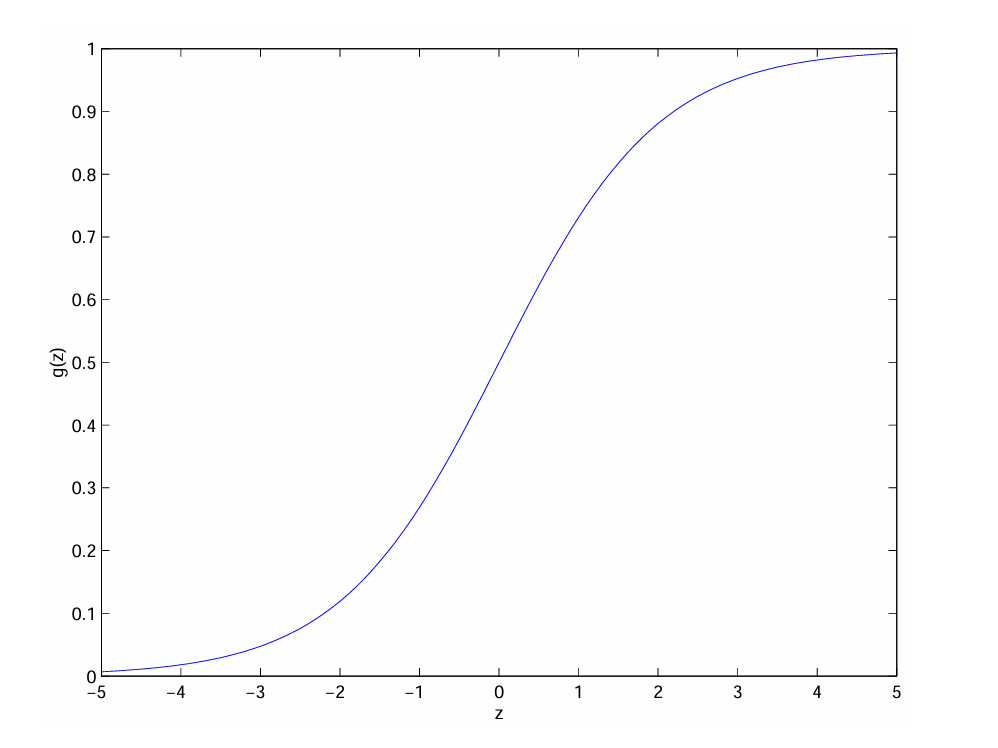
\includegraphics[width = 0.8\textwidth]{Figures/Sigmoid.png}
\end{center}

$\theta^{T}x$ is a linear transformation of the input $x$. Moreover, $g(z)$, and hence alse $h(x)$, 
is always bounded between 0 and 1. We are trying to map the input to a range of 0 to 1, representing 
the probability that the input belongs to the given label.

Other functions that smoothly increase from 0 to 1 can also be used, but for a couple of reasons that we'll see later 
(when we talk about GLMs, and when we talk about generative learning algorithms), the choice of the logistic function is a fairly natural one. 
Before moving on, here's a useful property of the derivative of the sigmoid function:
\begin{align*}
	g'(z) & = \frac{d}{dz} \frac{1}{1+e^{-z}}\\
	      & = \frac{1}{(1+e^{-z})^2} (e^{-z})\\
		  & = \frac{1}{1+e^{-z}} \left(1-\frac{1}{1+e^{-z}}\right)\\
		  & = g(z)\left(1-g(z)\right)
\end{align*}

\subsubsection{Logistic Loss Function}

Previously we introduce the cost function of linear regression as follows
\begin{equation*}
	J(\boldsymbol{\theta}) = \frac{1}{2m} \sum_{i=1}^{m} \left(h(x^{(i)})-y^{(i)}\right)^2
\end{equation*}

then write it in another way:

\begin{equation}
	J(\boldsymbol{\theta}) = \frac{1}{2} \sum_{i=1}^{m} \frac{1}{m} \left(h(x^{(i)})-y^{(i)}\right)^2
\end{equation}

We regard the part to the right of the summation symbol as a whole, called \textbf{the loss on a single training example}.
\begin{equation*}
	L\left(h(x^{(i)}), y^{(i)}\right)
\end{equation*}

As for the linear regression part, it's ok to use the previous form, meanly because that is a convex function for $J(\boldsymbol{\theta})$.
However, because of the introduction of logistic function, the previous form will lead to a non-convex function like this:

\begin{center}
	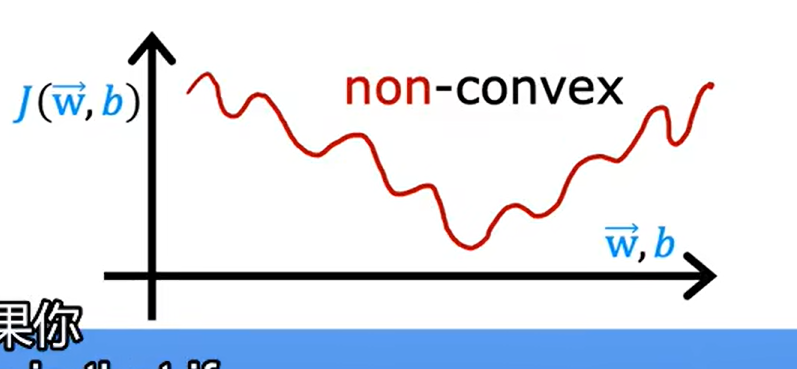
\includegraphics[width = 0.8\textwidth]{Figures/nonconvex.png}
\end{center}

It's hard to converge.
WE NEED TO INTRODUCE ANOTHER FORM!

\begin{equation}
	L\left(h(x^{(i)}), y^{(i)}\right) = 
	\begin{cases}
		-\ln(h(x^{(i)})) & \text{if } y^{(i)} = 1\\
		-\ln(1 - h(x^{(i)})) & \text{if } y^{(i)} = 0\\
	\end{cases}
\end{equation}

For the first equation that $y^{(i)} = 1$, here is the plot.
\begin{center}
	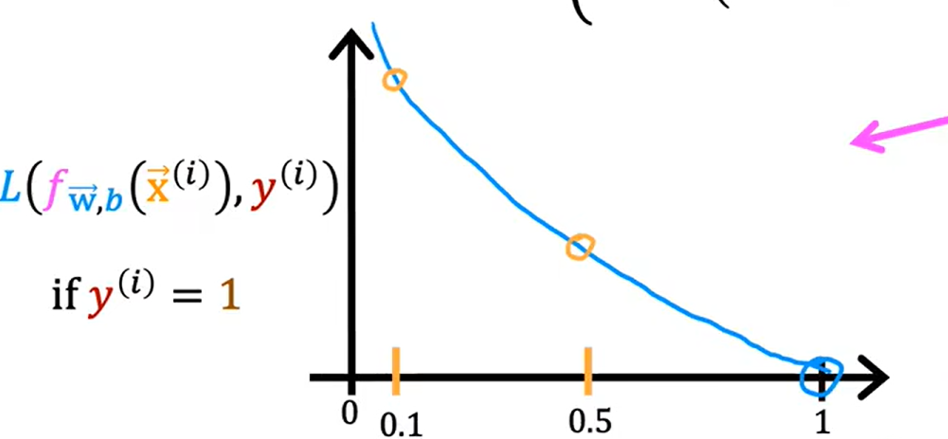
\includegraphics[width = 0.8\textwidth]{Figures/FirstPlot.png}
\end{center}

\begin{center}
	As $h(x^{(i)}) \to 1 \quad \text{then loss} \to 0$\\
	As $h(x^{(i)}) \to 0 \quad \text{then loss} \to 1$
\end{center}

It fulfils that loss is lowest when $h(x^{(i)})$ predict close to true label $y^{(i)}$.

For the first equation that $y^{(i)} = 1$, here is the plot.
\begin{center}
	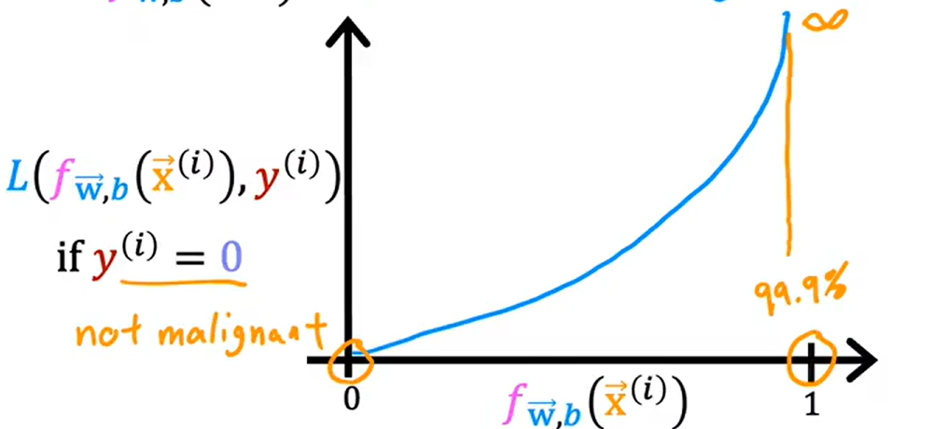
\includegraphics[width = 0.8\textwidth]{Figures/SecondPlot.png}
\end{center}

\begin{center}
	As $h(x^{(i)}) \to 0 \quad \text{then loss} \to 0$\\
	As $h(x^{(i)}) \to 1 \quad \text{then loss} \to 1$
\end{center}

The further prediction $h(x^{(i)})$ is from target $y^{(i)}$, the higher the loss.

This is what we actually want to use as the part of the new cost function. Notice both two of them are easy to converge.
Let's simplify cost function.

The loss function can be represented as the following form:
\begin{equation*}
	L\left(h(x^{(i)}), y^{(i)}\right) = -y^{(i)}\ln(h(x^{(i)})) - (1-y^{(i)})\ln(1-h(x^{(i)}))
\end{equation*}

Thus the final cost function:
\begin{equation}
	\begin{aligned}
	J(\boldsymbol{\theta}) & = \frac{1}{m} \sum_{i=1}^{m} \left[L\left(h(x^{(i)}), y^{(i)}\right)\right] \\
	& = -\frac{1}{m} \sum_{i=1}^{m} \left[y^{(i)}\ln(h(x^{(i)})) + (1-y^{(i)})\ln(1-h(x^{(i)}))\right]
	\end{aligned}
\end{equation}

The equation above is derived from \textbf{the maximum likelihood}, we'll talk about it later.

\subsubsection{Gradient Descent}
We can derived the formula as following from cost function. (However the process is a tiny little complex, I don't want to type them out)
\begin{equation*}
	\frac{\partial}{\partial \boldsymbol{\theta}_j} J(\boldsymbol{\theta}) 
	= \frac{1}{m} \sum_{i=1}^{m} \left(h(x^{(i)})-y^{(i)}\right) x^{(i)}_{j}
\end{equation*}
Surprise! It seems like it's the same with the former one.\\
But in fact, is it?
NO! They have different $h(\boldsymbol{x})$.

\begin{equation*}
	\begin{cases}
		\text{Linear regression} \quad h(\boldsymbol{x}) = \boldsymbol{\theta}^{T} \boldsymbol{x}\\
		\text{Logistic regression} \quad h(\boldsymbol{x}) = \frac{1}{1+e^{(\boldsymbol{\theta}^{T} \boldsymbol{x})}}
	\end{cases}
\end{equation*}

This therefore gives us the gradient descent rule
\begin{equation}
	\boldsymbol{\theta}_j = \boldsymbol{\theta}_j + \alpha \frac{1}{m} \sum_{i=1}^{m} \left[\left(y^{(i)} - h(x^{(i)})\right) x^{(i)}_{j}\right]
\end{equation}

The form is the same as the former, except for $h(\boldsymbol{x})$. Is this coincidence, or is there a deeper reason behind this? We'll answer this
when get get to GLM models.

\subsubsection{Again: Probabilistic Interpretation}
Let's assume that
\begin{equation*}
	\begin{aligned}
		P(y = 1 \arrowvert x; \theta) & = h(x)\\
		P(y = 0 \arrowvert x; \theta) & = 1- h(x)
	\end{aligned}
\end{equation*}
which can be written compactly as
\[
	p(y \arrowvert x;\theta) = \left(h(x)\right)^y \left(1-h(x)\right)^{1-y}
\]

Assuming that the m training examples were generated independently, we can then write down the likelihood 
of the parameters as
\begin{equation*}
	\begin{aligned}
		L(\theta) & = p(y \arrowvert x;\theta)\\
		          & = \prod_{i=1}^{m} p(y^{(i)} \arrowvert x^{(i)};\theta)\\
				  & = \prod_{i=1}^{m} \left(h(x^{(i)})\right)^{y^{(i)}} \left(1-h(x^{(i)})\right)^{1-y^{(i)}}
	\end{aligned}
\end{equation*}
As before, it will be easier to maximize the log likelihood:
\begin{equation*}
	\begin{aligned}
		\ell(\theta) & = \ln L(\theta)\\
		             & = \sum_{i=1}^{m} y^{(i)}\ln(h(x^{(i)})) + (1-y^{(i)})\ln(1-h(x^{(i)}))
	\end{aligned}
\end{equation*}

To maximize it, namely minimize the previous one. Here the proof is!

\subsection{Generalized Linear Models}
We can figure out that there are some somehow similarities between linear regression and classification regression. In this section, we will
show  that both of these methods are special cases of a broader family of models, called Generalized Linear Models (GLMs). We will also show 
how other models in the GLM family can be derived and applied to other classification and regression problems.

\subsubsection{The Exponential Family}
We say that a class of distributions is in the exponential family if it can be written in the form
\begin{equation}
	p(y;\eta) = b(y) \exp\left(\eta^{T}T(y) - a(\eta)\right)
\end{equation}

\begin{center}
	$\eta$: \textbf{natural parameter}\\
	$T(y)$: \textbf{sufficient statistic}\\
	$a(\eta)$: \textbf{log partition function}
\end{center}
The quantity $e^{-a(\eta)}$ essentially plays the role of a normalization constant, that makes sure the distribution 
$p(y;\eta)$ sums/integrates over y to 1.

We see that the probability of $y$ is determined by parameter $\eta$, so a fixed choice of $T$, $a$ and $b$ defines a family of distributions;
as we vary $\eta$, we get different distributions within this family.

Considering the \textbf{Bernoulli distribution}, as we vary $\phi$, which will contribute to $\eta$, we obtain Bernoulli distribution with different means.

We write the Bernoulli distribution as:
\begin{equation*}
	\begin{aligned}
		p(y; \phi) & = \phi^{y} \left(1-\phi\right)^{1-y}\\
		           & = \exp\left(y\ln\phi + (1-y)\ln(1-\phi)\right)\\
				   & = \exp\left(\ln\left(\frac{\phi}{1-\phi}\right)y + \ln(1-\phi)\right)
	\end{aligned}
\end{equation*}
Thus, the natural parameter is given by $\eta = \ln(\phi/(1-\phi))$.
\begin{equation*}
	\begin{aligned}
		T(y) & = y\\
		a(\phi) & = -\ln(1-\phi)\\
				& = \ln(l+e^{\phi})\\
		b(\phi) & = 1
	\end{aligned}
\end{equation*}

Let's now move on to consider the \textbf{Gaussian distribution}. Recall that when deriving linear regression, the value of $\sigma^2$
had no effect on our final choice of $\theta$. To simplify the derivation below, we set $\sigma^2 = 1$
\begin{equation*}
	\begin{aligned}
		p(y ; \mu) & =\frac{1}{\sqrt{2 \pi}} \exp \left(-\frac{1}{2}(y-\mu)^{2}\right) \\
		& =\frac{1}{\sqrt{2 \pi}} \exp \left(-\frac{1}{2} y^{2}\right) \cdot \exp \left(\mu y-\frac{1}{2} \mu^{2}\right)
		\end{aligned}
\end{equation*}
Thus, we see that the Gaussian is in the exponential family.
\begin{equation*}
	\begin{aligned}
		\eta & =\mu \\
		T(y) & =y \\
		a(\eta) & =\mu^{2} / 2 \\
		& =\eta^{2} / 2 \\
		b(y) & =(1 / \sqrt{2 \pi}) \exp \left(-y^{2} / 2\right)
		\end{aligned}
\end{equation*}



\end{document}

